Un générateur de tension, de force électromotrice $E$ alimente un conducteur
ohmique de résistance $R=\qty{100}{\ohm}$ et un condensateur de capacité $C$.
Un oscilloscope numérique est utilisé pour suivre l'évolution temporelle des
deux tensions en voie~1 et en voie~2
(Fig.~\ref{fig:2bac_svt_national_2024_rattrapage_phys_ex2_1}).

Le condensateur étant préalablement déchargé. À l'instant ${t_{0}=0}$, on ferme
l'interrupteur $\mathrm{K}$. Les évolutions temporelles des deux tensions sont
traduites par les courbes données par la
Fig.~\ref{fig:2bac_svt_national_2024_rattrapage_phys_ex2_2}.

\begin{minipage}{0.48\linewidth}
    \begin{figure}[H]
        \centering
        \begin{circuitikz}
            \newdimen\d \d=3cm
            \draw (0,0) coordinate (A)
                node[left] {$\mathrm{A}$}
                to[vsource,v=$E$,*-] ++(0,\d)
                to[cute open switch,l_=$\mathrm{K}$,-*] ++(\d,0) coordinate (D)
                node[above] {$\mathrm{D}$}
                to[R,l=$R$,-*] ++(0,-\d) coordinate (B)
                node[below] {$\mathrm{B}$}
                to[C,l=$C$,i>_=$i$] (A);
            \node[eground] at (A) {};
            \draw[-Triangle] (D) -- +(0.6,0) node[right] {Voie~1};
            \draw[-Triangle] (B) -- +(0.6,0) node[right] {Voie~2};
        \end{circuitikz}
        \caption{}
        \label{fig:2bac_svt_national_2024_rattrapage_phys_ex2_1}
    \end{figure}
\end{minipage}
\hfill
\begin{minipage}{0.48\linewidth}
    \begin{figure}[H]
        \centering
        \colorlet{majorgridcolor}{black}
        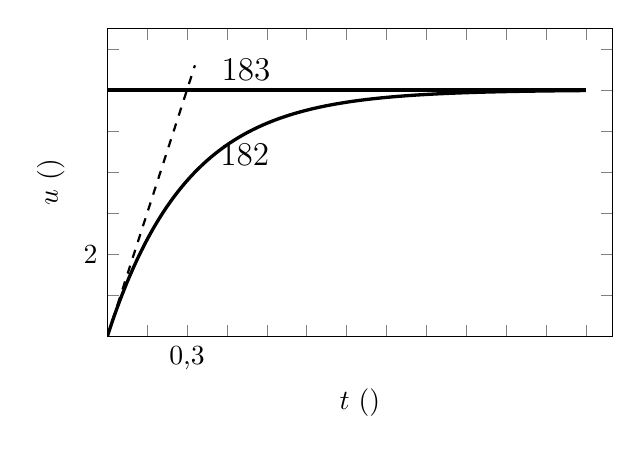
\begin{tikzpicture}
            \def\A{6}
            \def\ta{0.3}
            \begin{axis}[
                    samples=200,
                    xmin=0,xmax=1.9,
                    ymin=0,ymax=7.5,
                    width=8cm,height=5.5cm,
                    xtick distance=0.15,
                    ytick distance=1,
                    xlabel={$t~(\unit{\ms})$},
                    ylabel={$u~(\unit{\volt})$},
                    minor tick  num=0,
                    xticklabels={,,,0{,}3},
                    yticklabels={,,,2},
                ]
                \addplot[
                        domain=0:1.8,
                        very thick,black
                        ] {\A*(1-exp(-\x/\ta))}
                        coordinate[pos=0.73](C1);
                \addplot[
                        domain=0:0.33,
                        black,thick,dashed
                    ] {\A*\x/\ta)};
                \addplot[
                        domain=0:1.8,
                        very thick,black
                    ] {\A} coordinate[pos=0.29](C2);
            \end{axis}
            \node[below,font=\large] at (C1) {\ding{182}};
            \node[above,font=\large] at (C2) {\ding{183}};
        \end{tikzpicture}
        \caption{}
        \label{fig:2bac_svt_national_2024_rattrapage_phys_ex2_2}
    \end{figure}
\end{minipage}

\begin{enumerate}
    \item Recopier sur votre copie le schéma de la
          Fig.~\ref{fig:2bac_svt_national_2024_rattrapage_phys_ex2_1} et
          représenter, en convention récepteur, la tension $u_{C}$ aux bornes du
          condensateur et la tension $u_{R}$ aux bornes du conducteur
          ohmique.~\textbf{(1pt)}
    \item Parmi les courbes \ding{182} et \ding{183} de la
          Fig.~\ref{fig:2bac_svt_national_2024_rattrapage_phys_ex2_2}, quelle
          est celle qui correspond à la tension $u_{C}$~?
          Justifier.~\textbf{(1pt)}
    \item Montrer que l'équation différentielle vérifiée par la tension $u_{C}$
          s'écrit~:
          $RC\frac{\mathrm{d}u_{C}}{\mathrm{d}t}+u_{C}=E$.~\textbf{(1pt)}
    \item En admettant que $u_{c}=A\bigl(1-e^{-\frac{t}{\tau}}\bigr)$ est
          solution de l'équation différentielle.
          \begin{enumerate}
              \item Déterminer les expressions de $A$ et $\tau$ en fonction des
                    paramètres du circuit.~\textbf{(1pt)}
              \item Déterminer graphiquement les valeurs de $E$ et
                    $\tau$.~\textbf{(1pt)}
              \item En déduire la valeur de $C$.~\textbf{(1pt)}
          \end{enumerate}
    \item L'expression de l'intensité $i(t)$ du courant qui traverse le circuit
          est~:~\textbf{(1pt)}

          \begin{minipage}{\linewidth}
          \begin{table}[H]
              \centering
              \setlength{\arrayrulewidth}{0.8pt}
              \renewcommand{\arraystretch}{1.3}
              \begin{tabularx}{\textwidth}{|
                  >{\arraybackslash\centering}p{6mm}|C|
                  >{\arraybackslash\centering}p{6mm}|C|}
              \hline
              $\mathrm{A}$ & $i(t)=0,06\cdot e^{-3333,3\cdot t}~(\unit{\A})$
              &
              $\mathrm{B}$ & $i(t)=-0,06\cdot e^{-3333,3\cdot t}~(\unit{\A})$ \\
              \hline
              $\mathrm{C}$ & $i(t)=0,6\cdot e^{-3333,3\cdot t}~(\unit{\A})$
              &
              $\mathrm{D}$ & $i(t)=6\cdot e^{-3333,3\cdot t}~(\unit{\A})$ \\
              \hline
              \end{tabularx}
          \end{table}
          \end{minipage}
\end{enumerate}


